\chapter{Definitions}

In this chapter, we will cover the basic definitions and concepts related to complex networks. We will start with fundamental graph concepts, then explore various network representations, discuss graph isomorphism and permutation, and finally delve into connectedness, distances, subgraphs, planarity, homomorphism, network reduction, and spectral analysis of networks.

\section{Basic Graph Concepts}

We are going to start with the most basic definition of a graph, which serves as the foundation for all subsequent concepts in network theory. To introduce the concept of a graph, we will use the following definition:

\begin{definition}[Graph]
    A graph $G(V,L)$ is a finite nonempty set $V$ of $p$ points (vertexes or nodes) and a set of $k$ couples of distinct points $L$ (links, lines, or edges).
\end{definition}

From this definition, the concept of a graph is quite general and can be applied to a wide range of systems. The nodes can represent various entities such as people, computers, or proteins, while the links can represent relationships, interactions, or connections between these entities. The flexibility of this definition allows us to model complex systems in various fields, including social networks, communication networks, biological networks, and many others. There are some general rules that we typically follow when working with graphs, which are important to keep in mind as we explore more complex network structures.

\begin{remark}[General Rules]
    \begin{itemize}
        \item In general, networks have no loops (self-connections).
        \item There are no multigraphs, meaning no multiple links between the same nodes.
        \item We can, however, consider multiple links as weights or as multiple layers (multiplex).
    \end{itemize}
\end{remark}

\subsection{Directed and Undirected Graphs}
Directed graphs (DiGraphs) are graphs with directed edges, known as arcs, indicating a ``\textbf{from-to}'' \textbf{relationship}. They are used to describe hierarchical relationships, fluxes, or the passing of messages and goods. Undirected graphs contain only symmetric links and are used to describe symmetrical relations such as friendship, chemical bonds, or statistical correlation. Note that directed graphs can be symmetrized; while this loses some information, it allows the use of simpler properties and algorithms.

\subsection{Walk, Trail, Path, and Cycle}

Let us consider a graph with nodes $i$ and $j$. We can define different types of connections between these nodes:
\begin{itemize}
    \item \textbf{Walk}: A node and edge sequence between two nodes.
    \item \textbf{Trail}: A walk with all distinct links.
    \item \textbf{Path}: A walk with all distinct nodes and links.
    \item \textbf{Cycle}: A closed path with $N_c \ge 3$ nodes.
\end{itemize}
This classification is important for understanding the structure of networks and for defining concepts such as connectedness and distances. Different algorithms are used to find walks, trails, paths, and cycles in a graph, which can be crucial for applications like network traversal, routing, and community detection.

\section{Network Representations}

It is important to note that a graph can be represented in various ways, each with its own advantages and disadvantages. The choice of representation often depends on the specific application and the properties of the graph being studied.

\subsection{Adjacency Matrix}

The most common representation of a graph is the adjacency matrix, which is a square matrix that encodes the presence or absence of links between nodes. For unweighted graphs, the entries are binary (0 or 1), while for weighted graphs, the entries can take on a range of values corresponding to the weights of the links.

\begin{definition}[Adjacency Matrix]
    The adjacency matrix $A$ is an $N \times N$ matrix representing $N$ nodes. For unweighted networks, $A_{ij}=1$ indicates a topological link from node $i$ to node $j$, with $A_{ii}=0$ to indicate no loops. For weighted networks, $A_{ij}=w_{ij}$ where $w_{ij}$ is the weight of the link.
\end{definition}

\begin{minipage}{0.45\textwidth}
    \textbf{Directed Graph}

    Consider the following directed graph with 6 nodes, we can represent it with the following adjacency matrix:
    \begin{figure}[H]
        \centering
        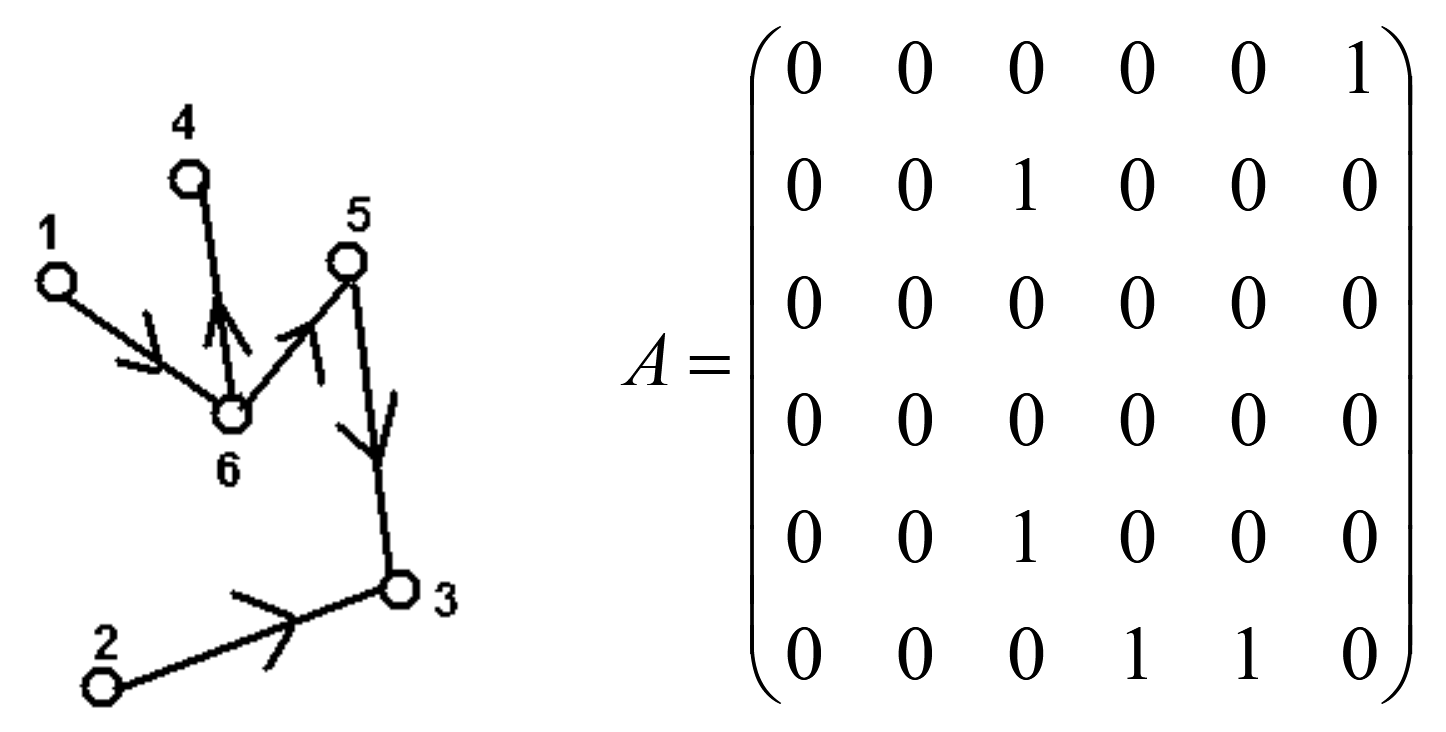
\includegraphics[width=\textwidth]{img/generic_adjacency.png}
        \caption{A directed graph and its corresponding non-symmetric adjacency matrix.}
    \end{figure}
\end{minipage}
\hfill
\begin{minipage}{0.45\textwidth}
    \textbf{Undirected Graph}

    Consider the following undirected graph with 6 nodes, we can represent it with the following adjacency matrix:
    \begin{figure}[H]
        \centering
        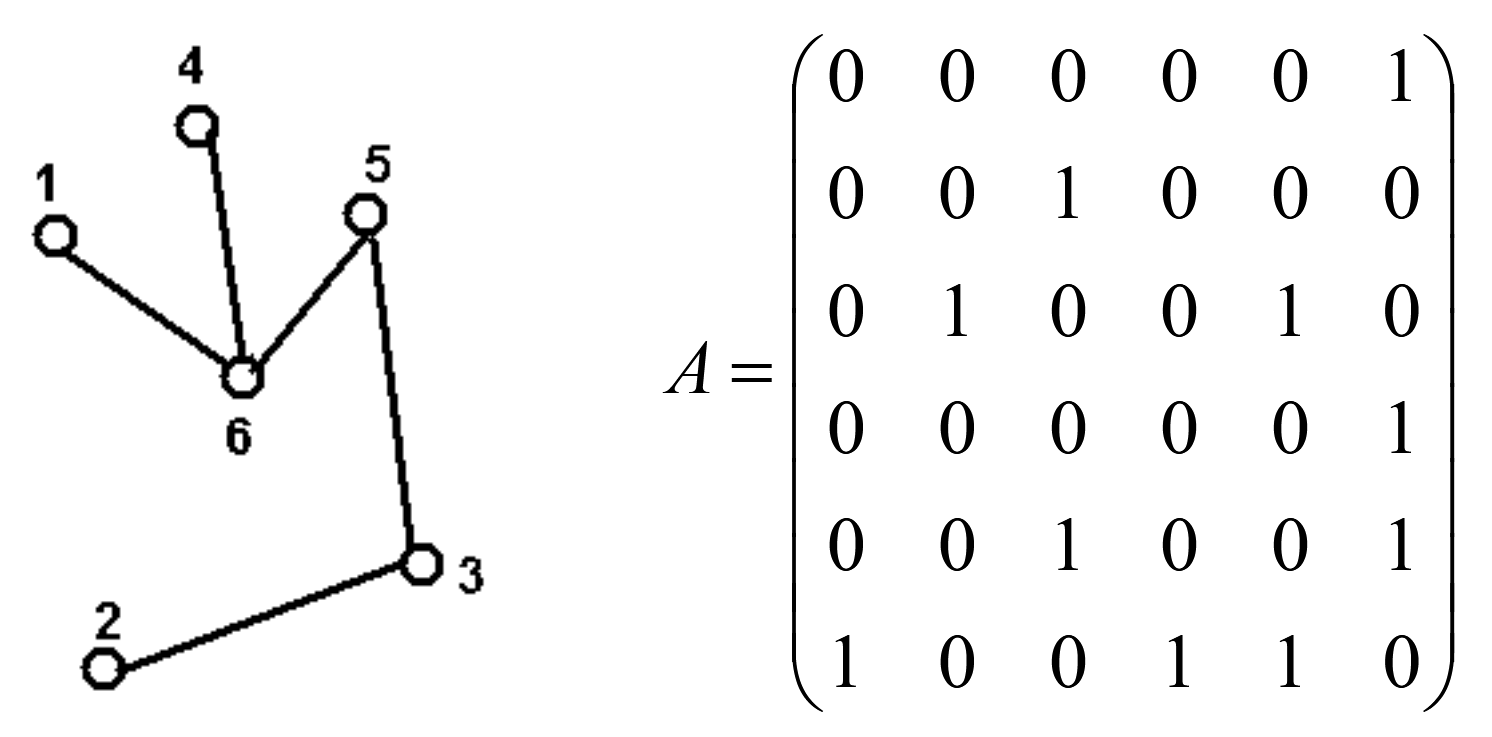
\includegraphics[width=\textwidth]{img/symmetric_adjacency.png}
        \caption{An undirected graph and its corresponding symmetric adjacency matrix.}
    \end{figure}
\end{minipage}

\begin{remark}[Logical Operators on Adjacency Matrices]
    We can apply element-wise logical operators on adjacency matrices:
    \begin{itemize}
        \item Network symmetrization uses a logical OR: $A' = \max(A, A^T) = A \cup A^T$.
        \item Identifying reciprocal links uses a logical AND: $A'' = \min(A, A^T) = A \cap A^T$.
        \item Identifying strictly directed links uses logical XOR: $XOR(A, A^T)$.
    \end{itemize}
\end{remark}

\subsection{Weighted Network}

In a weighted network, the adjacency matrix contains values that represent the strength of the connections between nodes:
\[
    A_{ij} = w_{ij} \text{ link from node } i \text{ to node } j \text{ with weight } w_{ij}.
\]
This can be interpreted in various ways depending on the context, such as the number of interactions, the intensity of relationships, or the capacity of links.

It can be seen as a representation of a \textbf{multigraph} with N multi-edges: \(w_{ij} = N\). If all weights are positive, we have useful theorems for matrices with positive values (Perron-Frobenius theorem) and we can connect to ``physical'' situations (transition probabilities of diffusion processes)
Negative weights can be meaningful too: in \textbf{signed networks} the sign of the weight can represent different types of relationships or interactions, such as:
\begin{itemize}
    \item \textbf{Friend-enemy}: in social networks, positive weights can represent friendships while negative weights can represent enmity.
    \item \textbf{Attraction-repulsion}: in physical systems, positive weights can represent attractive forces while negative weights can represent repulsive forces.
    \item \textbf{Ferromagnetic-antiferromagnetic}: in spin systems, positive weights can represent ferromagnetic interactions while negative weights can represent antiferromagnetic interactions.
\end{itemize}

One can also operate a weighted matrix symmetrization:
\begin{itemize}
    \item Average symmetrization: $A' = \frac{1}{2}(A + A^T)$.
    \item Random matrix symmetrization: $A' = \frac{1}{\sqrt{2}}(A + A^T)$.
\end{itemize}

\subsection{Incidence Matrix}

We can also represent a graph using an incidence matrix, which is an alternative to the adjacency matrix. The incidence matrix is particularly useful for certain types of analyses, such as flow problems and network dynamics.

\begin{definition}[Incidence Matrix]
    The incidence matrix $I$ of a graph $G(V,L)$ is an $L \times V$ matrix (number of links by number of vertexes). It contains $-1$ for outgoing connections and $+1$ for ingoing connections:
    \[
        \text{if } A_{ij} \neq 0, \quad I_{Ni} = \mp 1, \quad I_{Nj} = \pm 1.
    \]
    It can be interpreted as a ``generalized derivative'' on the graph, giving the oriented difference between values on adjacent nodes. If there is no preferred direction, we can use an unsigned incidence matrix with $I_{Ni} = 1$ for all links. It has to be read as if each link is a vector pointing from the source node to the target node, and the incidence matrix encodes the direction and magnitude of these vectors.
\end{definition}

Thus the incidence matrix can be used to analyze the flow of information or resources through the network, and it is particularly useful for studying directed graphs and their properties. The incidence matrix can also be used to derive the adjacency matrix through the relation $A = I^T I - D$, where $D$ is a diagonal matrix that accounts for the degree of each node.

\subsubsection{Generalized Derivative}

The incidence matrix can be interpreted as a generalized derivative on the graph, giving the oriented difference between values on adjacent nodes. The incidence matrix allows us to compute the net flow into or out of each node, which is essential for understanding the dynamics of processes.

Given a vector of values \(\mathbf{f}_i\) for each node, the incidence matrix \(I\) applied on the vector gives:
\[
    \begin{aligned}
        \sum_{j} I_{ij} \cdot \mathbf{f}_j & = \Delta_i,                                                  \\
        \Delta_i                           & = \mathbf{f}_i - \mathbf{f}_j \forall \text{adjacent nodes},
    \end{aligned}
\]
where \(\Delta_i\) represents the net flow into or out of node \(i\) based on the values of its neighbors. This interpretation is crucial for analyzing diffusion processes, random walks, and other dynamic phenomena on networks.

Geometrically, a network acts as a spatial structure: while a regular lattice discretizes Euclidean space, a complex graph represents a more intricate manifold. However, one must be careful, as the properties of this discrete manifold do not necessarily hold in the continuous limit.

\subsection{Sparse Representations}
For sparse graphs where the number of links is much smaller than $V^2$, other representations are preferred:
\begin{itemize}
    \item \textbf{Edge Matrix}: An $L \times 2$ matrix that stores single links instead of the full matrix. It is more efficient for sparse graphs, but it does not allow for fast access to neighbors. It is way less memory-consuming for sparse graphs:
          \[
              L = o(V^2) \quad \implies \quad 2\times L \ll V^2.
          \]
          It is useful for algorithms that need to iterate over links, such as those used in community detection or clustering.
    \item \textbf{Adjacency List}: Each line describes a node and contains the indices of its arrival nodes. This is particularly useful for diffusion processes, such as simulating random walks on a graph, but it has a higher memory cost than the edge matrix, since it requires storing the neighbors of each node and the same link is stored twice (once for each node it connects).
\end{itemize}

\begin{example}{Sparse Graph Representations}
    Let us consider a sparse graph with 6 nodes and 4 links. The adjacency matrix representation would require a $6 \times 6$ matrix, which contains many zeros, while the edge matrix would only require a $4 \times 2$ matrix to store the links. The adjacency list would also be more efficient in this case, as it would only need to store the neighbors of each node, rather than the full matrix. Explicitly:
    \[
        A = \begin{pmatrix}
            0 & 1 & 0 & 0 & 0 & 0 \\
            1 & 0 & 1 & 0 & 0 & 0 \\
            0 & 1 & 0 & 0 & 0 & 0 \\
            0 & 0 & 0 & 0 & 1 & 0 \\
            0 & 0 & 0 & 1 & 0 & 1 \\
            0 & 0 & 0 & 0 & 1 & 0
        \end{pmatrix}, \qquad I = \begin{pmatrix}
            1 & 0 & 0 & 0 \\
            1 & 1 & 0 & 0 \\
            0 & 1 & 0 & 0 \\
            0 & 0 & 1 & 0 \\
            0 & 0 & 1 & 1 \\
            0 & 0 & 0 & 1
        \end{pmatrix}, \qquad E = \begin{pmatrix}
            1 & 2 \\
            2 & 3 \\
            4 & 5 \\
            5 & 6
        \end{pmatrix}, \qquad L : \begin{array}{l}
            1 \rightarrow \{2\}    \\
            2 \rightarrow \{1, 3\} \\
            3 \rightarrow \{2\}    \\
            4 \rightarrow \{5\}    \\
            5 \rightarrow \{4, 6\} \\
            6 \rightarrow \{5\}
        \end{array}
    \]
    where $A$ is the adjacency matrix, $I$ is the incidence matrix, $E$ is the edge matrix, and $L$ is the adjacency list. As we can see, the adjacency matrix contains many zeros, while the edge matrix and adjacency list are more compact representations of the same graph.
\end{example}

\subsubsection{Random Walks and Diffusion Processes}

The choice of representation can significantly impact the efficiency of algorithms for simulating random walks and diffusion processes on networks. For example, the adjacency list allows for efficient access to neighbors, which is crucial for simulating random walks, while the edge matrix can be more efficient for algorithms that need to iterate over links, such as those used in community detection or clustering.

To emulate a \textbf{random walk on a graph}, we can use the adjacency list to quickly access the neighbors of each node and determine the probabilities of transitioning from one node to another. This is particularly important for large, sparse graphs where the number of links is much smaller than $V^2$, as it allows for efficient memory usage and faster computations. The steps to follow for simulating a random walk on a graph using the adjacency list are as follows:
\begin{enumerate}
    \item Start at a randomly selected node (or a specific node if desired).
    \item At each step, use the adjacency list to find the neighbors of the current node.
    \item Randomly select one of the neighbors to transition to, based on the weights of the links (for a pure random walk we have to consider a uniform distribution, otherwise we could use the link weights/biases etc.).
    \item Repeat the process for a specified number of steps or until a certain condition is met (e.g., reaching a target node).
\end{enumerate}
This method allows us to efficiently simulate random walks and diffusion processes on large, sparse networks, which is essential for understanding the dynamics of complex systems.

\section{Graph Isomorphism and Permutation}

We are now going to discuss the concept of graph isomorphism, which is a fundamental notion in graph theory that describes when two graphs are essentially the same, even if they are represented differently.

\begin{definition}[Graph Isomorphism]
    An isomorphism is a 1-1 correspondence between vertexes that preserves the link structure. It corresponds to a node index permutation.
\end{definition}

This means that two graphs are isomorphic if there exists a permutation of the node labels of one graph that results in the adjacency matrix of the other graph. In other words, the two graphs have the same structure, but their nodes may be labeled differently. We have then to digress on the concept of node permutation and permutation matrix, which is a fundamental operation in graph theory that allows us to rearrange the nodes of a graph without changing its structure.

A permutation of the nodes of a graph can be represented by a permutation matrix, which is a square binary matrix that has exactly one entry of 1 in each row and each column, and 0s elsewhere. The permutation matrix can be used to rearrange the rows and columns of the adjacency matrix of a graph, effectively permuting the nodes. There exist \(N!\) possible permutations of the nodes, which means that there are \(N!\) different permutation matrix realising the isomorphism: each \(N\times N\) network can be represented by \(N!\) different adjacency matrices, all isomorphic.

The properties of the permutation matrix are as follows:
\[
    \begin{aligned}
        P \cdot P^T = \mathbb{I} \implies P^T = P^{-1} \quad & \text{(orthogonality)}                   \\
        P \cdot A \cdot P^T = A' \quad                       & \text{(adjacency matrix transformation)} \\
        \vert P \vert = \pm 1 \quad                          & \text{(determinant)}                     \\
    \end{aligned}
\]

\begin{remark}[Re-indexing]
    Node permutation represents node reordering, which is a common operation in graph algorithms. It allows us to rearrange the nodes of a graph without changing its structure, which can be useful for various applications such as community detection, clustering, and visualization. However, it is important to note that while node permutation can change the appearance of the adjacency matrix, it does not change the underlying properties of the graph, such as its degree distribution, clustering coefficient, or path lengths. Thus node re-indexing has to be made after gaining insights on the graph structure, thus it can be based on:
    \begin{itemize}
        \item \textbf{A priori information}: we can have information directly about the network, due to ontological knowledge of the system (e.g. known community structure or node attributes) or intrinsic metric properties of the graph (e.g., spatial networks, node proximity).
        \item \textbf{Network-based information}: we can have information about the network structure, such as node degree, centrality measures, or community structure, which can be used to reorder the nodes in a way that reveals patterns or simplifies the analysis.
    \end{itemize}
\end{remark}
These re-indexing strategies can help us to better understand the structure of the graph and to identify important features or patterns that may not be immediately apparent in the original representation. The \textbf{visualization} of a network can be significantly improved by reordering the nodes based on their properties or the structure of the graph, which can help to reveal hidden patterns and relationships between nodes (a chain network can be visualized as a sparse one if we make poor re-indexing choices).

\begin{example}[Protein and DNA Contact Maps]
    A network representation of peptide bonds serves as a discretization of a 3D distance matrix: a fully connected graph with weights given by the spatial distance between amino acids. The re-indexing of nodes can be based on the spatial proximity of amino acids, which can help to reveal patterns in the contact map and provide insights into the structure and function of the protein.

    Spatial closeness acts as an ``intrinsic'' metric for the graph. One can use the re-indexing in order to exploit different properties of the graph, such as symmetry or centrality measures, study spatial closeness, revealing the backbone of the network, or identify communities.

    DNA 3D structure can also be represented as a similar network, where nodes represent nucleotides and links represent spatial proximity or interactions between them. Re-indexing based on spatial proximity can help to reveal patterns in the contact map and provide insights into the structure and function of the DNA molecule (the hi-c technique is used to obtain such contact maps).
\end{example}

\section{Connectedness}

Studying the connectedness of a graph is crucial for understanding its structure and the dynamics of processes that occur on it. Connectedness refers to the extent to which nodes in a graph are connected to each other, and it can be classified into different types based on the nature of the connections.

\subsection{Undirected Graphs}
An undirected graph is \textbf{connected} if it is not divided into two or more non-communicating parts: from every node there is a path to every other node. If there are multiple disconnected components, the graph is called \textbf{disconnected}.
Algebraically, this means there is no permutation that reduces the adjacency matrix into diagonal blocks, it is not isomorphic to a block diagonal matrix
\[
    P A P^{-1} = \begin{pmatrix}
        A_1 & 0   \\
        0   & A_2
    \end{pmatrix}.
\]
The number of blocks corresponds to the number of disconnected components. Any matrix which can be transformed into a block form (diagonal or upper triangular) is called \textbf{reducible}, while a matrix that cannot be transformed into such a form is called \textbf{irreducible}.

It is important to notice that from the same dataset more then one graph can be constructed, depending on the definition of the links; even from the same adjacency matrix, different re-indexing can lead to different visualizations of the same graph, which can reveal different patterns and structures. But before any analysis, it is crucial to check the connectedness of the graph, as many properties and algorithms assume that the graph is connected. Some network properties rely on the assumption of connectedness, other than the components number and size, so it is a crucial information to have before starting any analysis.

\subsection{Directed Graphs}

In a directed graph, not every node is necessarily reachable from any other. After a \textbf{block matrix reduction}, we are often left with a block upper triangular matrix, where the blocks on the diagonal represent strongly connected components
\[
    P A P^{-1} = \begin{pmatrix}
        A_1 & B   \\
        0   & A_2
    \end{pmatrix}, \quad A_1 \xrightarrow{B} A_2, \quad A_1 \nleftarrow A_2.
\]
In this situation, we can say that block $A_1$ is \textbf{upstream} of block $A_2$, while block $A_2$ is \textbf{downstream} of block $A_1$. The presence of the block $B$ indicates that there are connections from nodes in block $A_1$ to nodes in block $A_2$, but not vice versa. This structure can have important implications for the dynamics of processes on the graph, such as diffusion or information flow.

In a directed graph, connectedness does not guarantee that every node is reachable from any other. It is classified into three types:
\begin{itemize}
    \item \textbf{Strongly connected}: Every node is connected to another by a path, implying the existence of cycles.
    \item \textbf{Unilaterally connected}: For every two nodes, there is at least one path (i.e. in one direction, as for the absorbing states seen before).
    \item \textbf{Weakly connected}: Every node is connected to another by at least a semipath.
\end{itemize}
Semi-paths, semi-walks etc. are defined as paths, walks etc. where it is necessary to traverse edges in an unspecified direction (we may need to reverse the direction of one or more links to complete the path). The presence of cycles in a directed graph is a key factor in determining whether the graph is strongly connected, as cycles allow for bidirectional connectivity between nodes.

We can also write three theorems about the connectedness of directed graphs:
\begin{itemize}
    \item Strongly connected implies that exists one spanning closed walk.
    \item Unilaterally connected implies that exists one spanning walk.
    \item Weakly connected implies that exists one spanning semiwalk.
\end{itemize}
All these theorems can be proved by contradiction, by assuming that there is no spanning walk and showing that this leads to a contradiction with the definition of connectedness.

\begin{figure}[H]
    \begin{minipage}{0.6\textwidth}
        \centering
        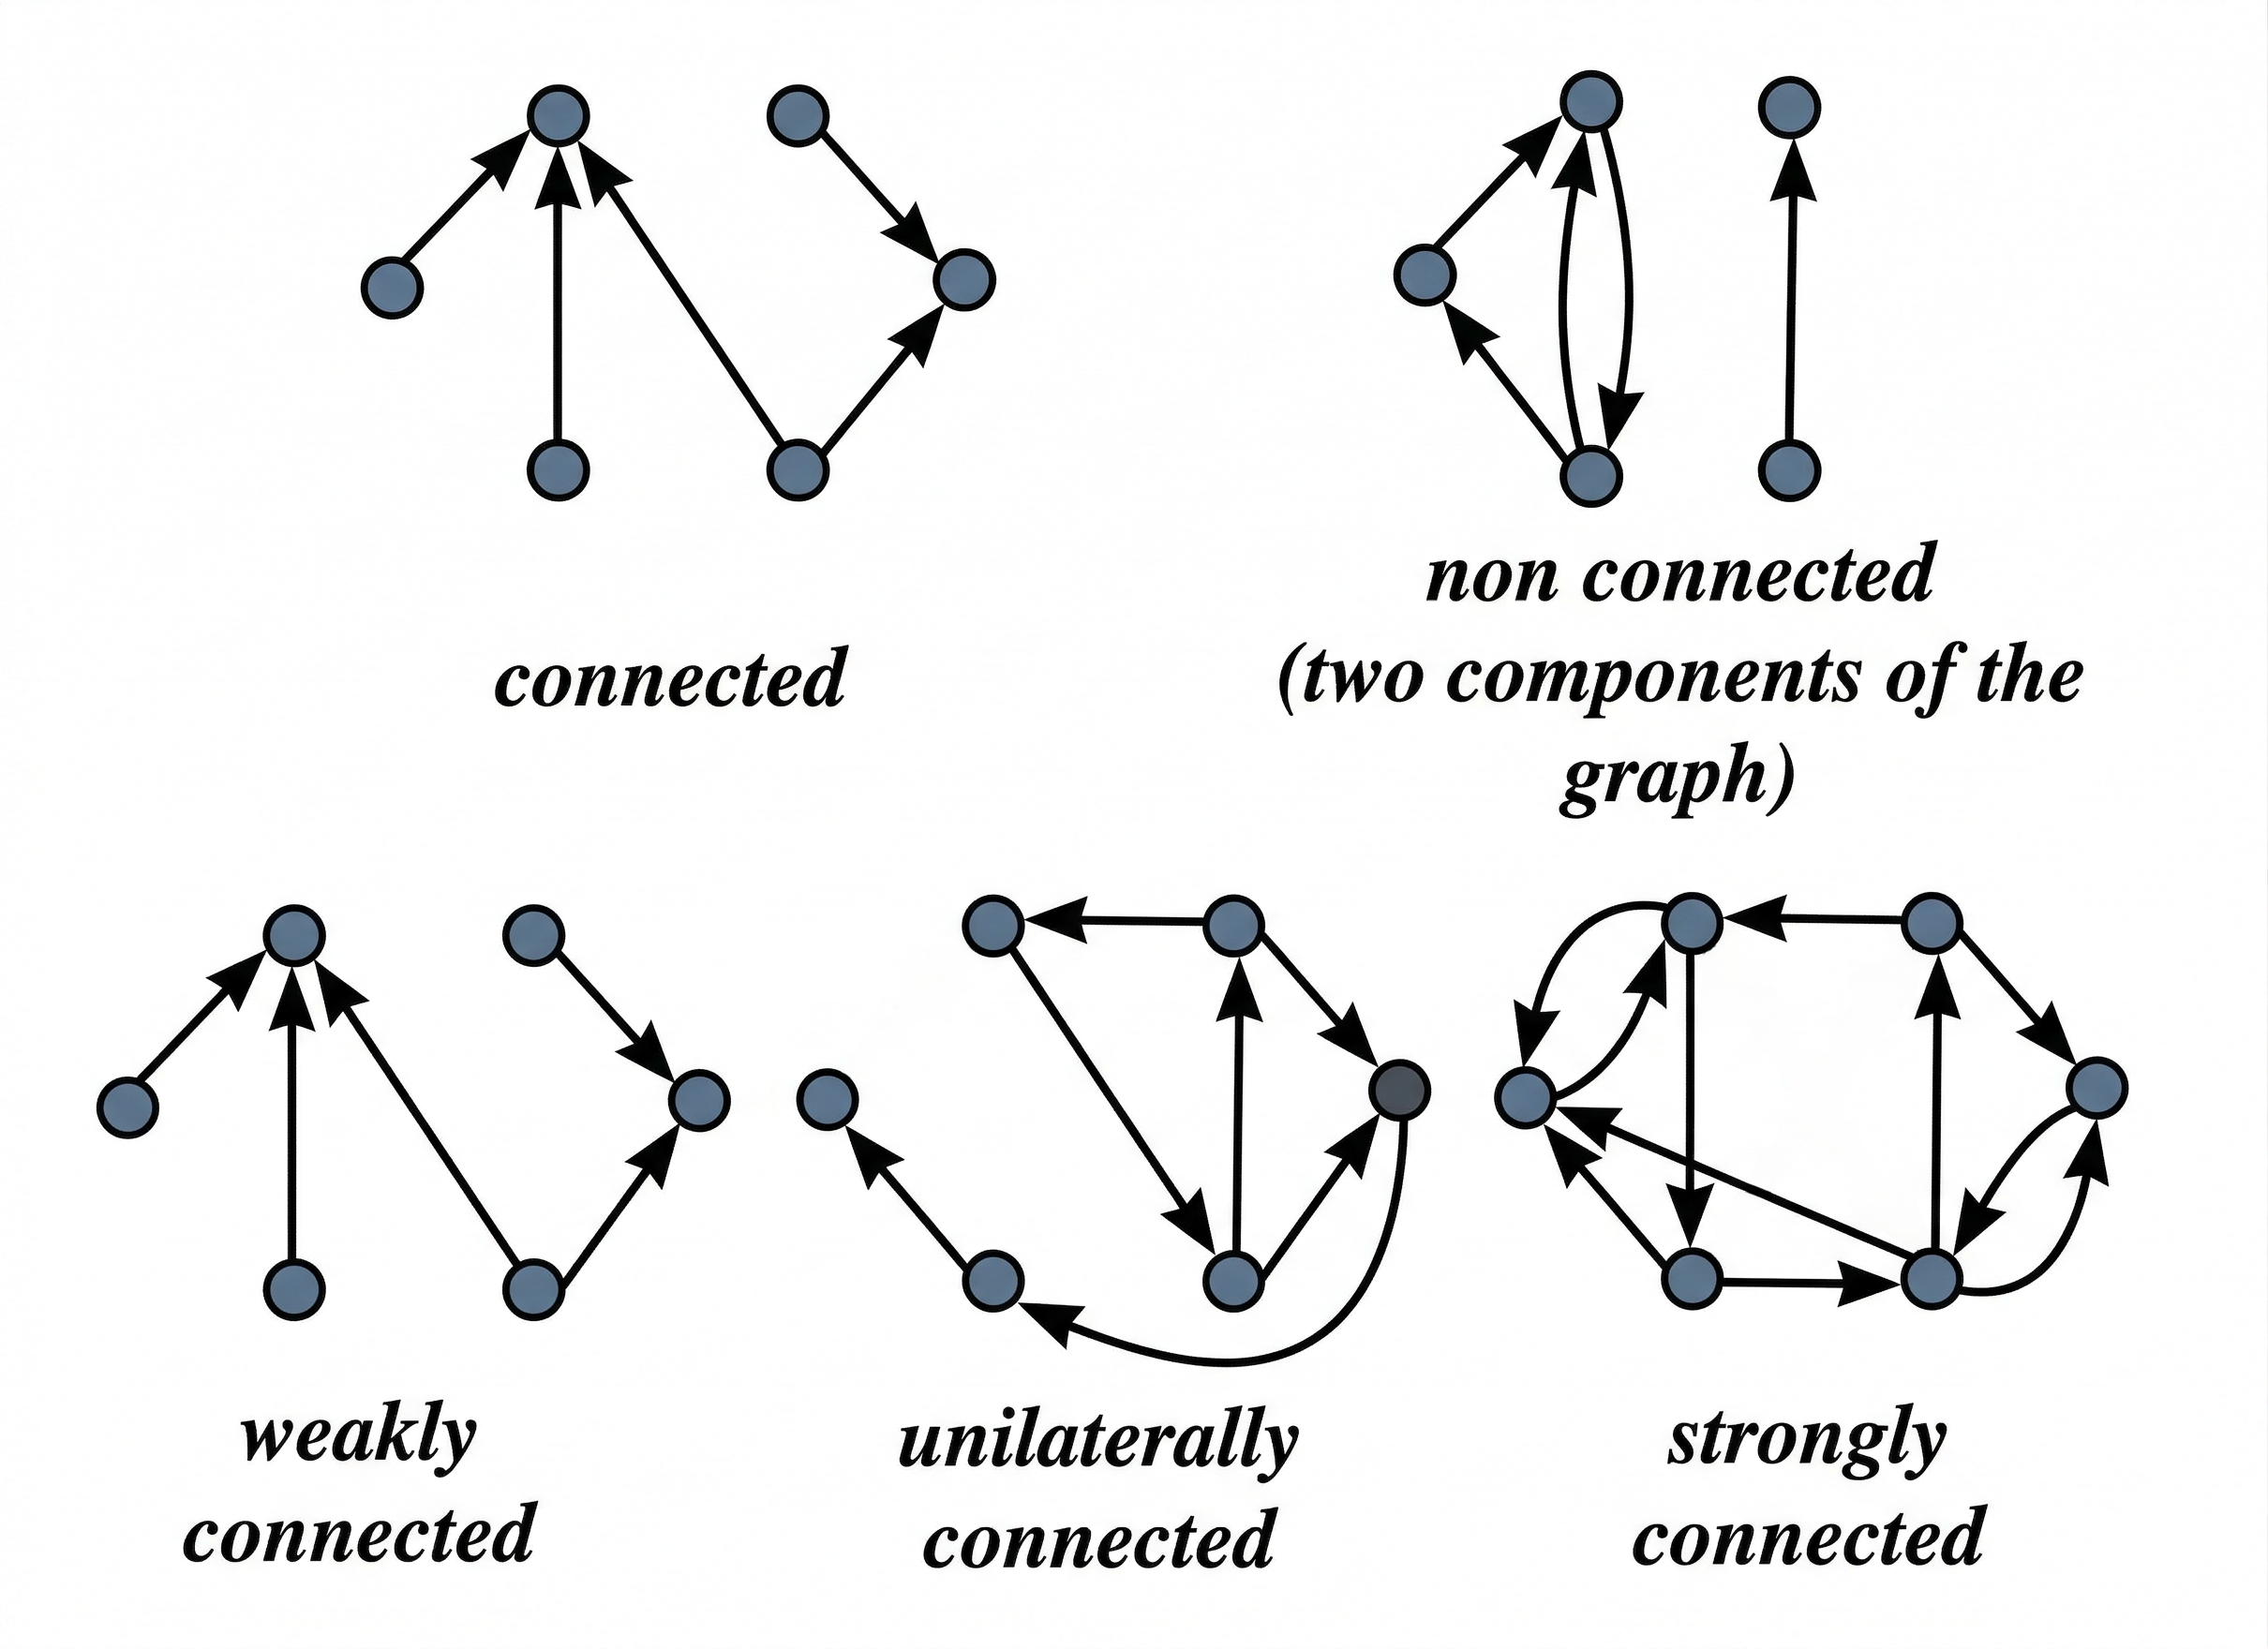
\includegraphics[width=\textwidth]{img/connectedness_examples.png}
    \end{minipage}
    \hfill
    \begin{minipage}{0.35\textwidth}
        \caption{Examples of different types of connectedness in directed graphs. The left graph is weakly connected (since there is a semipath between every pair of nodes), the middle graph is unilaterally connected (since there is at least one path between every pair of nodes), and the right graph is strongly connected (since every node is reachable from every other node with a path).}
    \end{minipage}
\end{figure}

\section{Distances and Shortest Paths}

We are now going to discuss the concept of distance in graphs, which is a fundamental notion that allows us to quantify how far apart nodes are from each other. The distance between two nodes can be defined in various ways, depending on the context and the type of graph being studied.

\subsection{Node Distance}
The distance between two nodes is defined as the shortest path between them. There are different ways to define distance, depending on the context and the type of graph:
\begin{itemize}
    \item \textbf{Unweighted distance}: The distance is the number of links in the shortest path between two nodes.
    \item \textbf{Weighted distance}: The distance is the sum of the weights of the links in the shortest path between two nodes.
\end{itemize}
Let us study more in detail each case.

\subsubsection{Unweighted Distance}

In unweighted networks, the distance between two nodes is simply the number of links in the shortest path connecting them. This is often referred to as the \textbf{geodesic distance}. The geodesic distance can be defined as
\begin{itemize}
    \item Isolated nodes have infinite distance from any other node: \(D(u,v) = \infty\) if there is no path between nodes \(u\) and \(v\).
    \item Adjacent nodes have a distance of 1: \(D(u,v) = 1\) if there is a link between nodes \(u\) and \(v\).
    \item A node is at distance 0 from itself: \(D(u,v) = 0\) if \(u = v\).
    \item The distance between two nodes is the minimum number of links in any path connecting them: \(D(u,v) = \min\{k : \text{there exists a path of length } k \text{ from } u \text{ to } v\}\).
\end{itemize}

Note that topologically, if we are defining a distance on a symmetric graph, we are defining a metric space, since the distance satisfies the properties of a metric:
\begin{enumerate}
    \item \textbf{Positive semidefiniteness}: \(D(u,v) \geq 0\) for all nodes \(u\) and \(v\), and \(D(u,v) = 0\) if and only if \(u = v\).
    \item \textbf{Symmetry}: \(D(u,v) = D(v,u)\) for all nodes \(u\) and \(v\).
    \item \textbf{Triangle inequality}: \(D(u,w) \leq D(u,v) + D(v,w)\) for all nodes \(u\), \(v\), and \(w\).
\end{enumerate}

One last remark is that one can define different types of distances, such as the distance between node embeddings, one with the overlap of \(n\) neighbors, or the distance between communities, which can be defined as the distance between their centroids in a suitable embedding space.

\subsubsection{Weighted Distance}

In weighted networks, nodes that are ``closer'' have a greater weight, and distance can be calculated using \textbf{harmonic composition} (similar to capacitors in series): if we have more path between two nodes, the shortest path is the one with the greatest weight. We can define the weighted distance as
\[
    d_{ij} = \sum_{i \to j} \frac{1}{w_{kl}},
\]
where the sum is taken over all paths from node \(i\) to node \(j\), and \(w_{kl}\) is the weight of the link between nodes \(k\) and \(l\) along the path. This definition allows us to capture the idea that stronger connections (higher weights) correspond to shorter distances, while weaker connections (lower weights) correspond to longer distances. If there is a zero-weight link, it can be interpreted as an infinite weight (i.e., no connection), which means that the distance between the nodes is infinite:
\[
    w = 0 \implies d \to \infty.
\]
\begin{example}
    The matrix of \textbf{Euclidean distances} \(d_{ij}\) between elements of a defined N-dim space, can be seen as a fully connected symmetric weighted network: every element is connected to every other element, and the weight of the link between two elements is given by the Euclidean distance between them. This representation can be useful for analyzing spatial relationships and clustering in data, as well as for visualizing high-dimensional data in a lower-dimensional space. For example, in a protein structure, we can represent the distances between amino acids as a weighted network, where nodes represent amino acids and links represent the spatial proximity between them. This can help us to understand the structure and function of the protein, as well as to identify important interactions between amino acids.

    Depending on the context, we can also define the distance as a function of the weights \(d_{ij} = f(w_{ij})\), where \(f\) is a suitable function that captures the relationship between weights and distances. For example, we could use an exponential decay function, or a logarithmic function, one based on gaussian kernels, etc. The choice of the function \(f\) would depend on the specific application and the properties of the data being analyzed.
\end{example}

\subsection{Shortest Path and Algorithms}
The distance between two nodes equals the minimum number of links (geodesic) between them. It is useful to define some auxiliary concepts:
\begin{itemize}
    \item \textbf{Eccentricity}: The maximum distance from a node to any other node in the graph.
    \item \textbf{Radius}: The minimum eccentricity among all nodes in the graph.
    \item \textbf{Diameter}: The maximum eccentricity among all nodes in the graph.
    \item \textbf{Average path length}: The average distance between all pairs of nodes in the graph.
\end{itemize}

The shortest path can be found using various algorithms, some of the most common ones include:
\begin{itemize}
    \item \textbf{Dijkstra's algorithm}: This algorithm is used for \textit{finding the shortest paths between nodes in a graph}, which may represent, for example, road networks. It works by iteratively selecting the node with the smallest tentative distance and updating the distances to its neighbors until the shortest path to the target node is found (one-to-all mechanism).
    \item \textbf{Floyd-Warshall algorithm}: This algorithm is used for \textit{finding the shortest paths between all pairs of nodes in a graph}. It works by iteratively updating a distance matrix based on the shortest paths found so far, until all pairs of nodes have been considered (all-to-all mechanism).
\end{itemize}
Both of these algorithms are implemented efficiently in every SW language (such as Python, C, R, Matlab etc.) and can be used to compute shortest paths in large graphs. The choice of algorithm depends on the specific requirements of the problem, such as whether we need to find the shortest path between a single pair of nodes or between all pairs of nodes.

\section{Subgraphs and Special Network Topologies}

We are going to discuss some special types of subgraphs and network topologies that are commonly studied in graph theory and network science. These structures can provide insights into the properties and dynamics of complex networks.

\begin{definition}[Subgraph, Spanning Subgraph, Induced Subgraph]
    \begin{itemize}
        \item \textbf{Subgraph}: A subset of a graph's nodes and links.
        \item \textbf{Spanning Subgraph}: A subgraph that contains all the nodes of the original graph (but not necessarily all the links).
        \item \textbf{Induced Subgraph}: A subset of the nodes of $G$ with ALL the links of $G$ that exist between those specific nodes.
    \end{itemize}
\end{definition}
\begin{figure}[H]
    \centering
    \begin{minipage}{0.8\textwidth}
        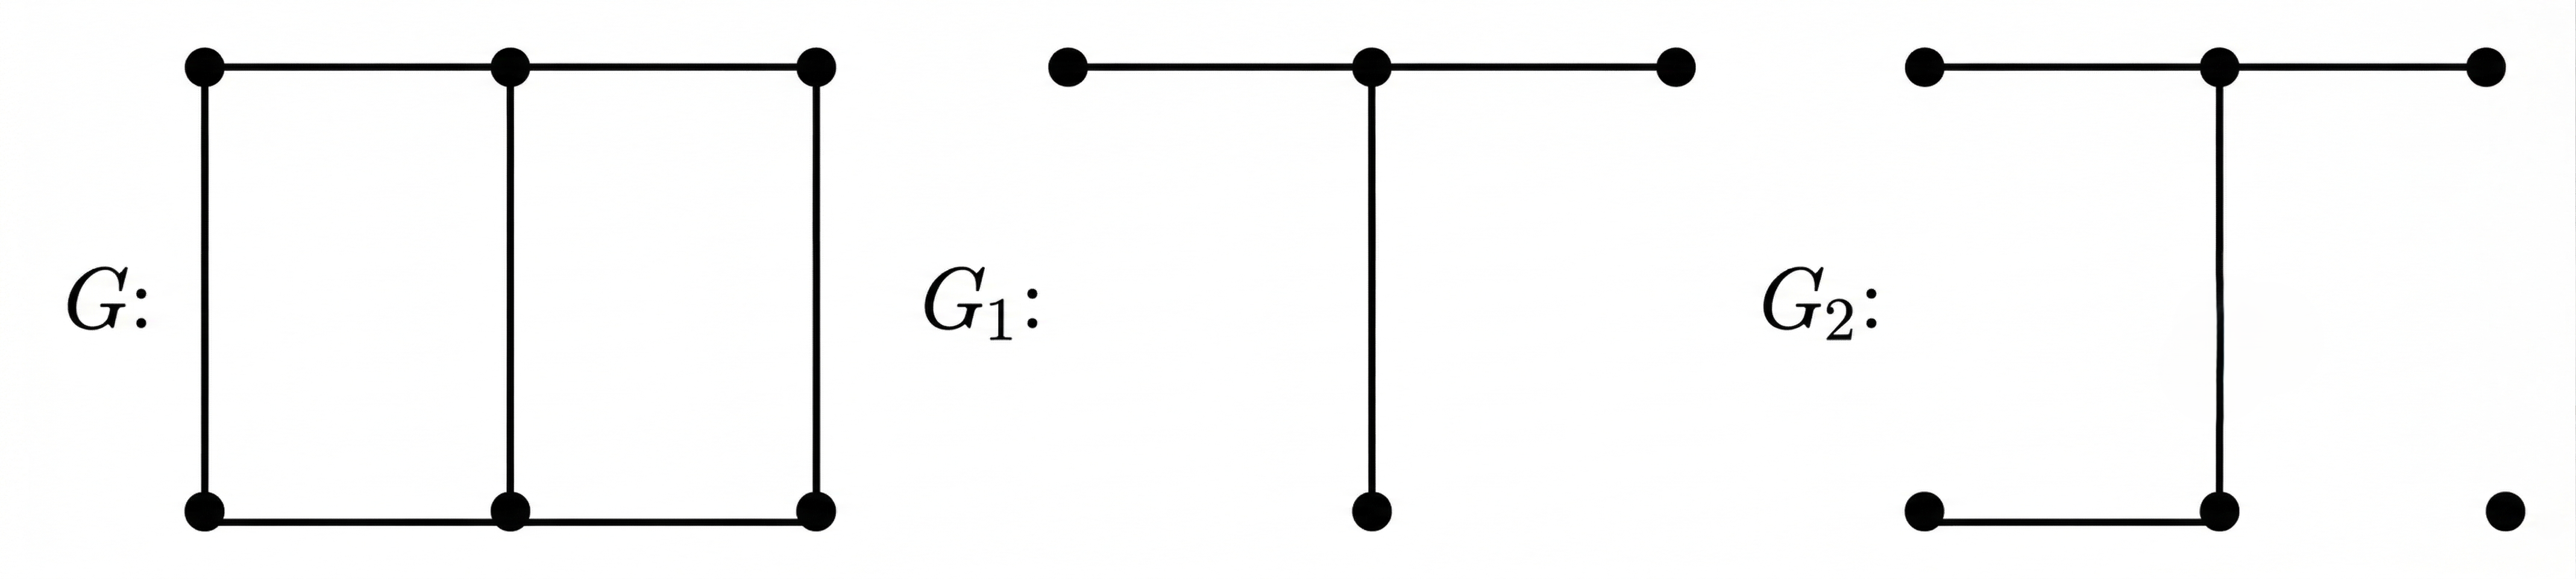
\includegraphics[width=\textwidth]{img/subgraphs_examples.png}
        \caption{Examples of different types of subgraphs. \(G\) is the original graph, \(G_1\) is an induced subgraph while \(G_2\) is a spanning subgraph.}
    \end{minipage}
\end{figure}

To extract the adjacency matrix of an induced subgraph $S$, you simply need to find the intersection of the rows and columns of the original matrix $A$ that correspond exactly to the nodes in $S$. Practically, removing elements from the network translates to very basic matrix operations:
\begin{itemize}
    \item \textbf{Node removal:} To remove a specific node $i$ from the network, you just delete the entire $i$-th row and the $i$-th column from the adjacency matrix $A$.
    \item \textbf{Link removal:} To remove the connection between node $i$ and node $j$, you simply set the matrix element $a_{ij}$ to $0$. If the graph is undirected (symmetric), you must also remove the reciprocal link by setting $a_{ji}$ to $0$.
\end{itemize}

\subsection{Complete Graphs, Complement, K-Cliques and Bipartite Graphs}

Let us now discuss some special types of graphs that are commonly studied in graph theory and network science, including complete graphs, graph complements, k-cliques and bipartite graphs.

\begin{definition}[Complete Graph]
    A completely connected graph $K_N$ with $N$ nodes with all possible links is called a \textbf{complete graph}, meaning every node has a degree of $K = N-1$:
    $$\# l = \binom{N}{2} = \frac{N!}{2!(N-2)!} = \frac{N(N-1)}{2}.$$
\end{definition}

\begin{definition}[Graph Complement and Self-Complementary]
    The \textbf{graph complement} is a network consisting of the exact same set of nodes, but with ``opposite'' connections. Specifically, two nodes are linked in the complement graph if and only if they were not linked in the original graph. Algebraically, if $A$ is the adjacency matrix of the original graph, the matrix of its complement can be calculated by applying $(A + 1) \pmod{2}$ to the elements (keeping the diagonal as zero).

    Furthermore, a graph is defined as \textbf{self-complementary} if it is isomorphic to its own complement. This means that, despite the links being inverted, the new network shares the exact same structural topology as the original one.
\end{definition}

\begin{definition}[K-Clique]
    A \textbf{K-clique} is a fully connected subgraph of $G$ with degree $K$. Finding a clique of a certain size in a graph, known as the \textbf{clique problem}, is NP-complete. This means it is computationally infeasible, as the complexity grows more than a power of the number of nodes.
\end{definition}

A strongly connected subgraph, such as a clique, can be seen as a \textbf{community} within the network, meaning its nodes are likely to share similar properties. While a single link in an adjacency matrix describes a simple 1-to-1 relationship, a clique can effectively represent an $N$-body relationship. Practical examples of such structures include protein complexes, chemical reactions, and other multi-body interactions.

\begin{definition}[Bipartite Graph]
    A graph that connects two different types of nodes between each other, but NOT between themselves. It is represented by an $M \times N$ rectangular adjacency matrix. In terms of matrix algebra, a bipartite graph is an imprimitive matrix of order 2.
\end{definition}

Thus in a bipartite graph, we have two distinct sets of nodes, and links only exist between nodes from different sets. This structure is common in many real-world networks, such as social networks (e.g., people and their affiliations), biological networks (e.g., genes and diseases), and information networks (e.g., users and items in a recommendation system).

In a complete bigraph every node of one type is connected to every node of the other type. The number of links in a biclique is given by $L = M \times N$, where $M$ and $N$ are the number of nodes in the two sets.

The \textbf{adjacency matrix} of a bipartite graph can be represented in block form as follows:
\[
    A = \begin{pmatrix}
        0   & B \\
        B^T & 0
    \end{pmatrix},
\]
where $B$ is an $M \times N$ matrix that represents the connections between the two sets of nodes. The upper left and lower right blocks are zero matrices, indicating that there are no connections between nodes of the same type.

\begin{figure}[H]
    \begin{minipage}{0.6\textwidth}
        \centering
        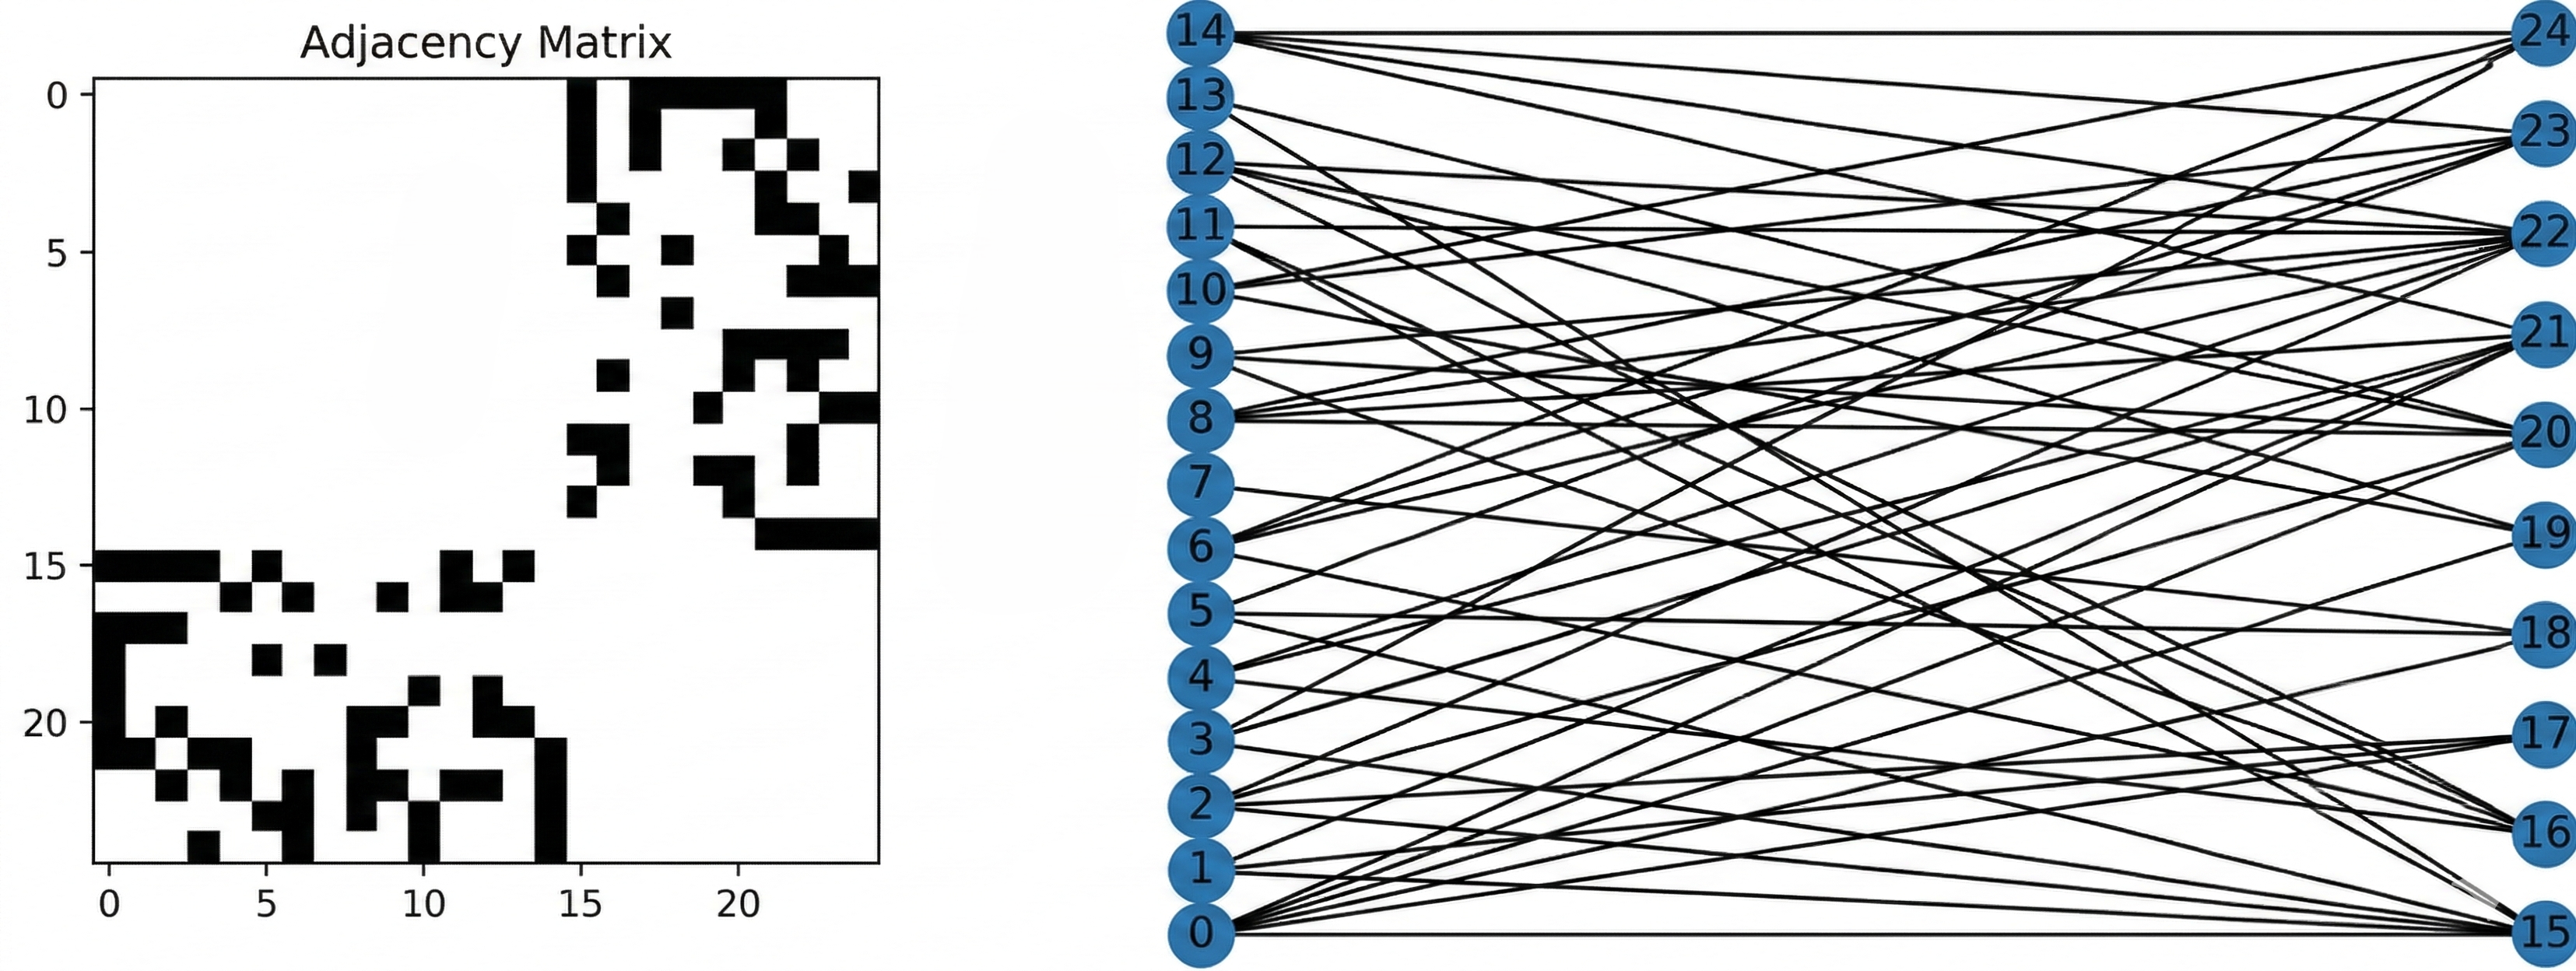
\includegraphics[width=\textwidth]{img/bipartite_graph_example.png}
    \end{minipage}
    \hfill
    \begin{minipage}{0.35\textwidth}
        \caption{An example of a bipartite graph and its corresponding block adjacency matrix; it is structured in a way that reflects the bipartite nature of the graph, with the off-diagonal blocks representing the connections between the two sets of nodes.}
    \end{minipage}
\end{figure}

\subsubsection{Primitivity and Imprimitivity}

When representing a bipartite graph with an $(M+N) \times (M+N)$ square adjacency matrix, we can always find a node permutation that neatly separates the two sets of nodes. This rearrangement leads to a block matrix structure featuring zero blocks on the main diagonal and two non-diagonal blocks representing the cross-connections: there exists a permutation matrix \(P\) such that
\[
    P A P^{-1} = \begin{pmatrix}
        0        & B^1_{mn} \\
        B^2_{nm} & 0
    \end{pmatrix}.
\]
In terms of matrix algebra, this specific block structure means the bipartite graph corresponds to an \textbf{imprimitive matrix of order 2}. Conceptually, traversing this network results in a continuous ``flip'' in node values as you alternate between the two distinct sets. A \textbf{primitive matrix} instead corresponds to a graph where there is a path of any length between any two nodes, without the need for such a flip, indicating a more interconnected structure.

This topological and algebraic concept can be generalized to higher dimensions: an \textbf{$N$-partite graph} corresponds exactly to an \textbf{$N$-imprimitive matrix}. By applying the appropriate node permutation, its adjacency matrix can be organized into a ``cyclic'' $N$-block array. In this configuration, all nodes within a given block are connected \textit{only} to nodes belonging to another specific block, and there are no connections between nodes within the same block. This structure leads to a continuous ``flip'' in node values as you traverse the network, cycling through the different blocks in a specific order.
\begin{figure}[H]
    \begin{minipage}{0.55\textwidth}
        \centering
        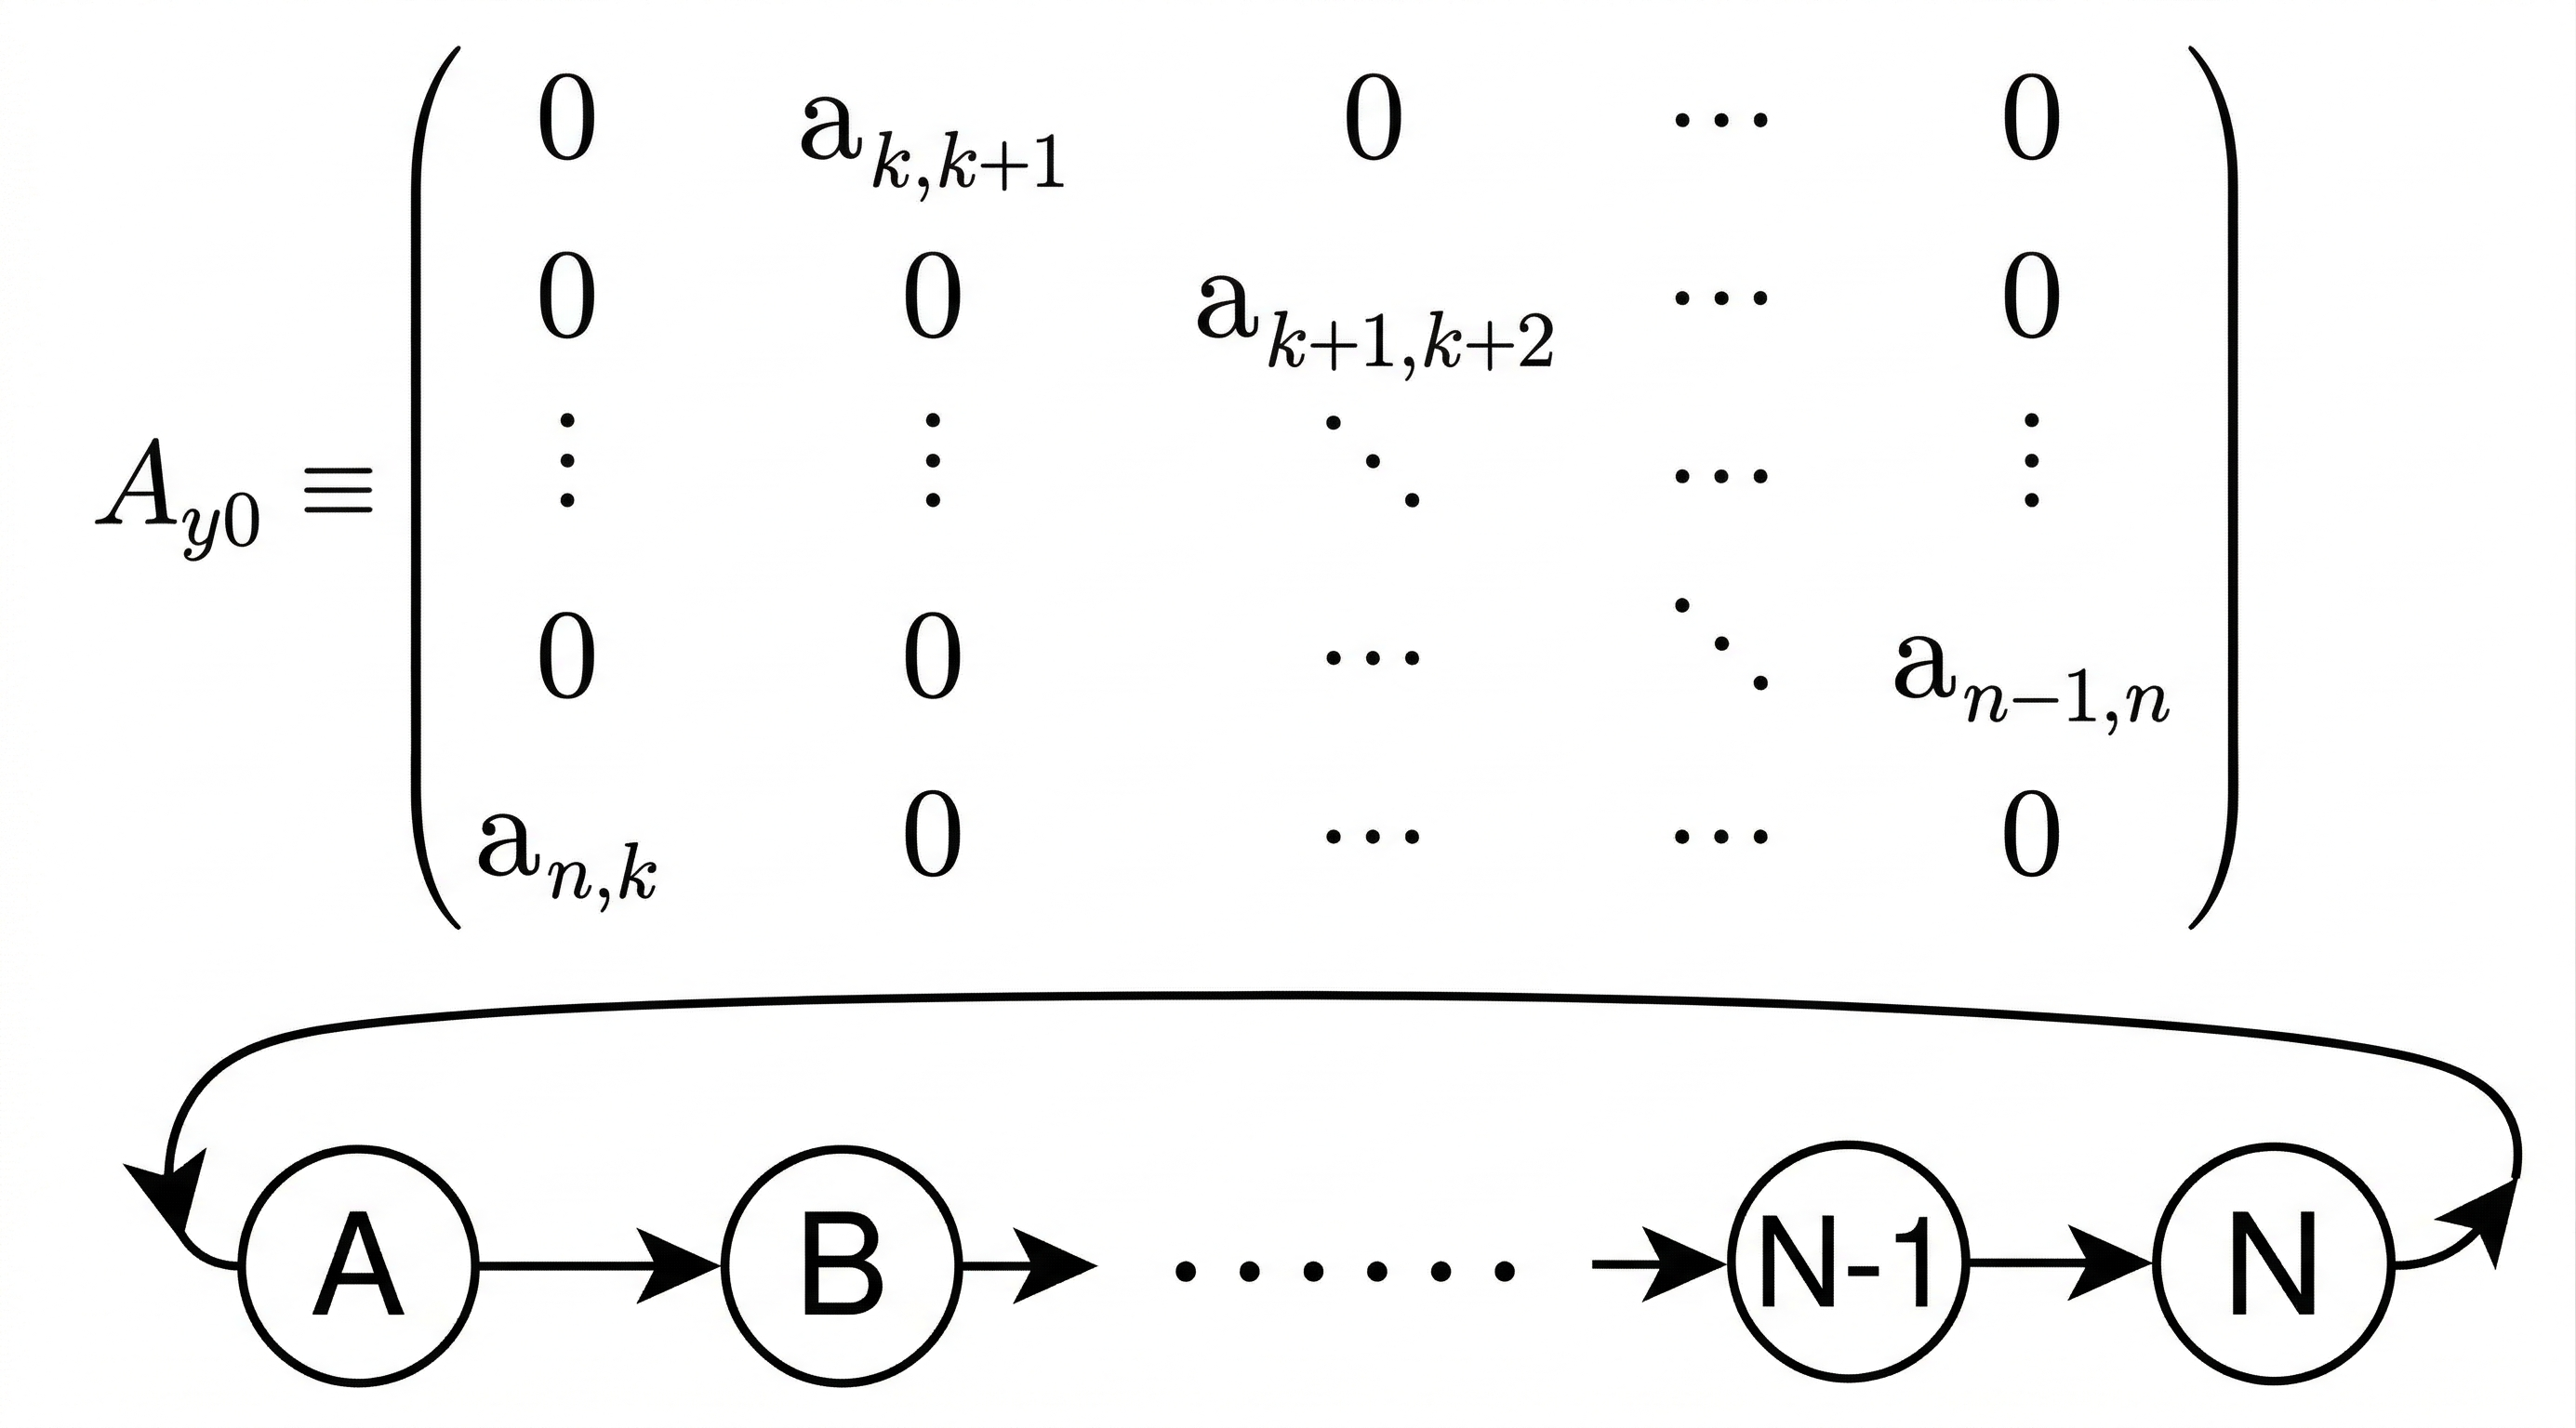
\includegraphics[width=\textwidth]{img/n_partite_graph_example.png}
    \end{minipage}
    \hfill
    \begin{minipage}{0.4\textwidth}
        \caption{An example of a n-partite graph and its corresponding block adjacency matrix; the adjacency matrix is structured in a way that reflects the n-partite nature of the graph, with the off-diagonal blocks representing the connections between the n sets of nodes.}
    \end{minipage}
\end{figure}
Determining whether a matrix is primitive or imprimitive is crucial in network analysis. \textbf{Primitivity} is a fundamental algebraic property required to apply several advanced mathematical theorems to networks, most notably the Perron-Frobenius theorem.

\subsubsection{Tensor Contraction}
Given the rectangular adjacency matrix $B$ of dimensions $M \times N$, we can perform a tensor contraction to obtain two distinct square networks that connect nodes of the same type. This is achieved through simple matrix multiplication:
\begin{itemize}
    \item An $M \times M$ matrix calculated as $B \cdot B^T$.
    \item An $N \times N$ matrix calculated as $B^T \cdot B$.
\end{itemize}

In both of these resulting matrices, two nodes of the same type are linked if there is at least one path between them through a node of the other type in the original bipartite graph. If we treat the new networks as weighted, the link weight corresponds exactly to the number of common nodes of the other type they share.

Common examples of this projection include co-authorship networks (authors connected by shared papers), actors in the same movie, genes related to the same diseases, or drugs acting on the same diseases.

\begin{remark}[Directed Graph Symmetrization]
    In addition to the standard topological symmetrization obtained by simply adding the matrix and its transpose ($A + A^T$), a directed graph represented by an $N \times N$ adjacency matrix $A$ can be projected into two distinct symmetric graphs, $B$ and $C$, using matrix multiplication.

    This process reveals hidden similarities between nodes based on their connection patterns:
    \begin{itemize}
        \item By computing \textbf{$B = A^T \cdot A$}, we connect two nodes if they both point to at least one common target node. This is widely known as ``bibliographic coupling''; for instance, two distinct research papers are linked if they cite the exact same reference in their bibliography.
        \item Conversely, by computing \textbf{$C = A \cdot A^T$}, we connect two nodes if they receive incoming links from at least one common source node. This represents ``co-citation coupling'', meaning two papers are linked if they are both cited by the exact same third paper.
    \end{itemize}
\end{remark}


\begin{example}[The Human Disease Network]
    An example of a bipartite graph is the ``diseasome'' (e.g., OMIM database), a gene-pathology network. By contracting the matrix, we can obtain a gene-gene network based on shared diseases, or a pathology-pathology network based on shared genes.

    Analyzing this projected disease network reveals several key medical insights:
    \begin{itemize}
        \item \textbf{Communities and connectivity:} Similar diseases (such as various types of cancers) share many genes and are therefore highly connected. As a result, diseases naturally form clustered communities based on organ-related proximity (e.g., heart, brain, or blood diseases) or functional similarities.
        \item \textbf{Unexpected topological results:} The network structure shows that, counterintuitively, not all organ-related diseases are connected. Furthermore, discovering unexpected links between seemingly unrelated diseases opens the door to \textbf{drug repurposing}—suggesting that a drug effective for one disease might also be applied to a connected, yet distinct, pathology.
        \item \textbf{Further analysis:} To extract deeper biological meaning, the network can be enriched by attaching additional ``labels'' to the nodes, such as disease mortality rates or the specific functional role of a gene within the cell.
    \end{itemize}
\end{example}

\subsection{Trees and Stars}

Let us now discuss some special types of tree-like structures that are commonly studied in graph theory and network science, including star networks and tree networks.

\subsubsection{Star Network}

The star network is a simple network topology where one central node is connected to all other nodes, which are not connected to each other. This structure resembles a star, with the central node acting as the \textbf{hub} and the other nodes as the \textbf{spokes}. The star network is characterized by its simplicity and efficiency in terms of communication, as all nodes can communicate with each other through the central hub. However, it also has a significant drawback: if the central node fails, the entire network becomes disconnected, as there are no alternative paths for communication between the peripheral nodes. The star network is often used in scenarios where a central authority or coordinator is needed, such as in certain types of organizational structures or in some communication networks. However, it is not suitable for large-scale networks or those that require high levels of redundancy and fault tolerance, due to its vulnerability to the failure of the central node.

\subsubsection{Tree Network}

A tree network is a hierarchical structure that consists of nodes connected in a \textbf{parent-child relationship}. It is a type of \textbf{acyclic graph} where each node has one parent and can have multiple children. The topmost node is called the root, and the nodes at the bottom are called leaves. Tree networks are commonly used in organizational structures, file systems, and decision-making processes. They allow for efficient data organization and retrieval but can become inefficient if the tree becomes too deep or unbalanced.
\begin{figure}[H]
    \begin{minipage}{0.45\textwidth}
        \centering
        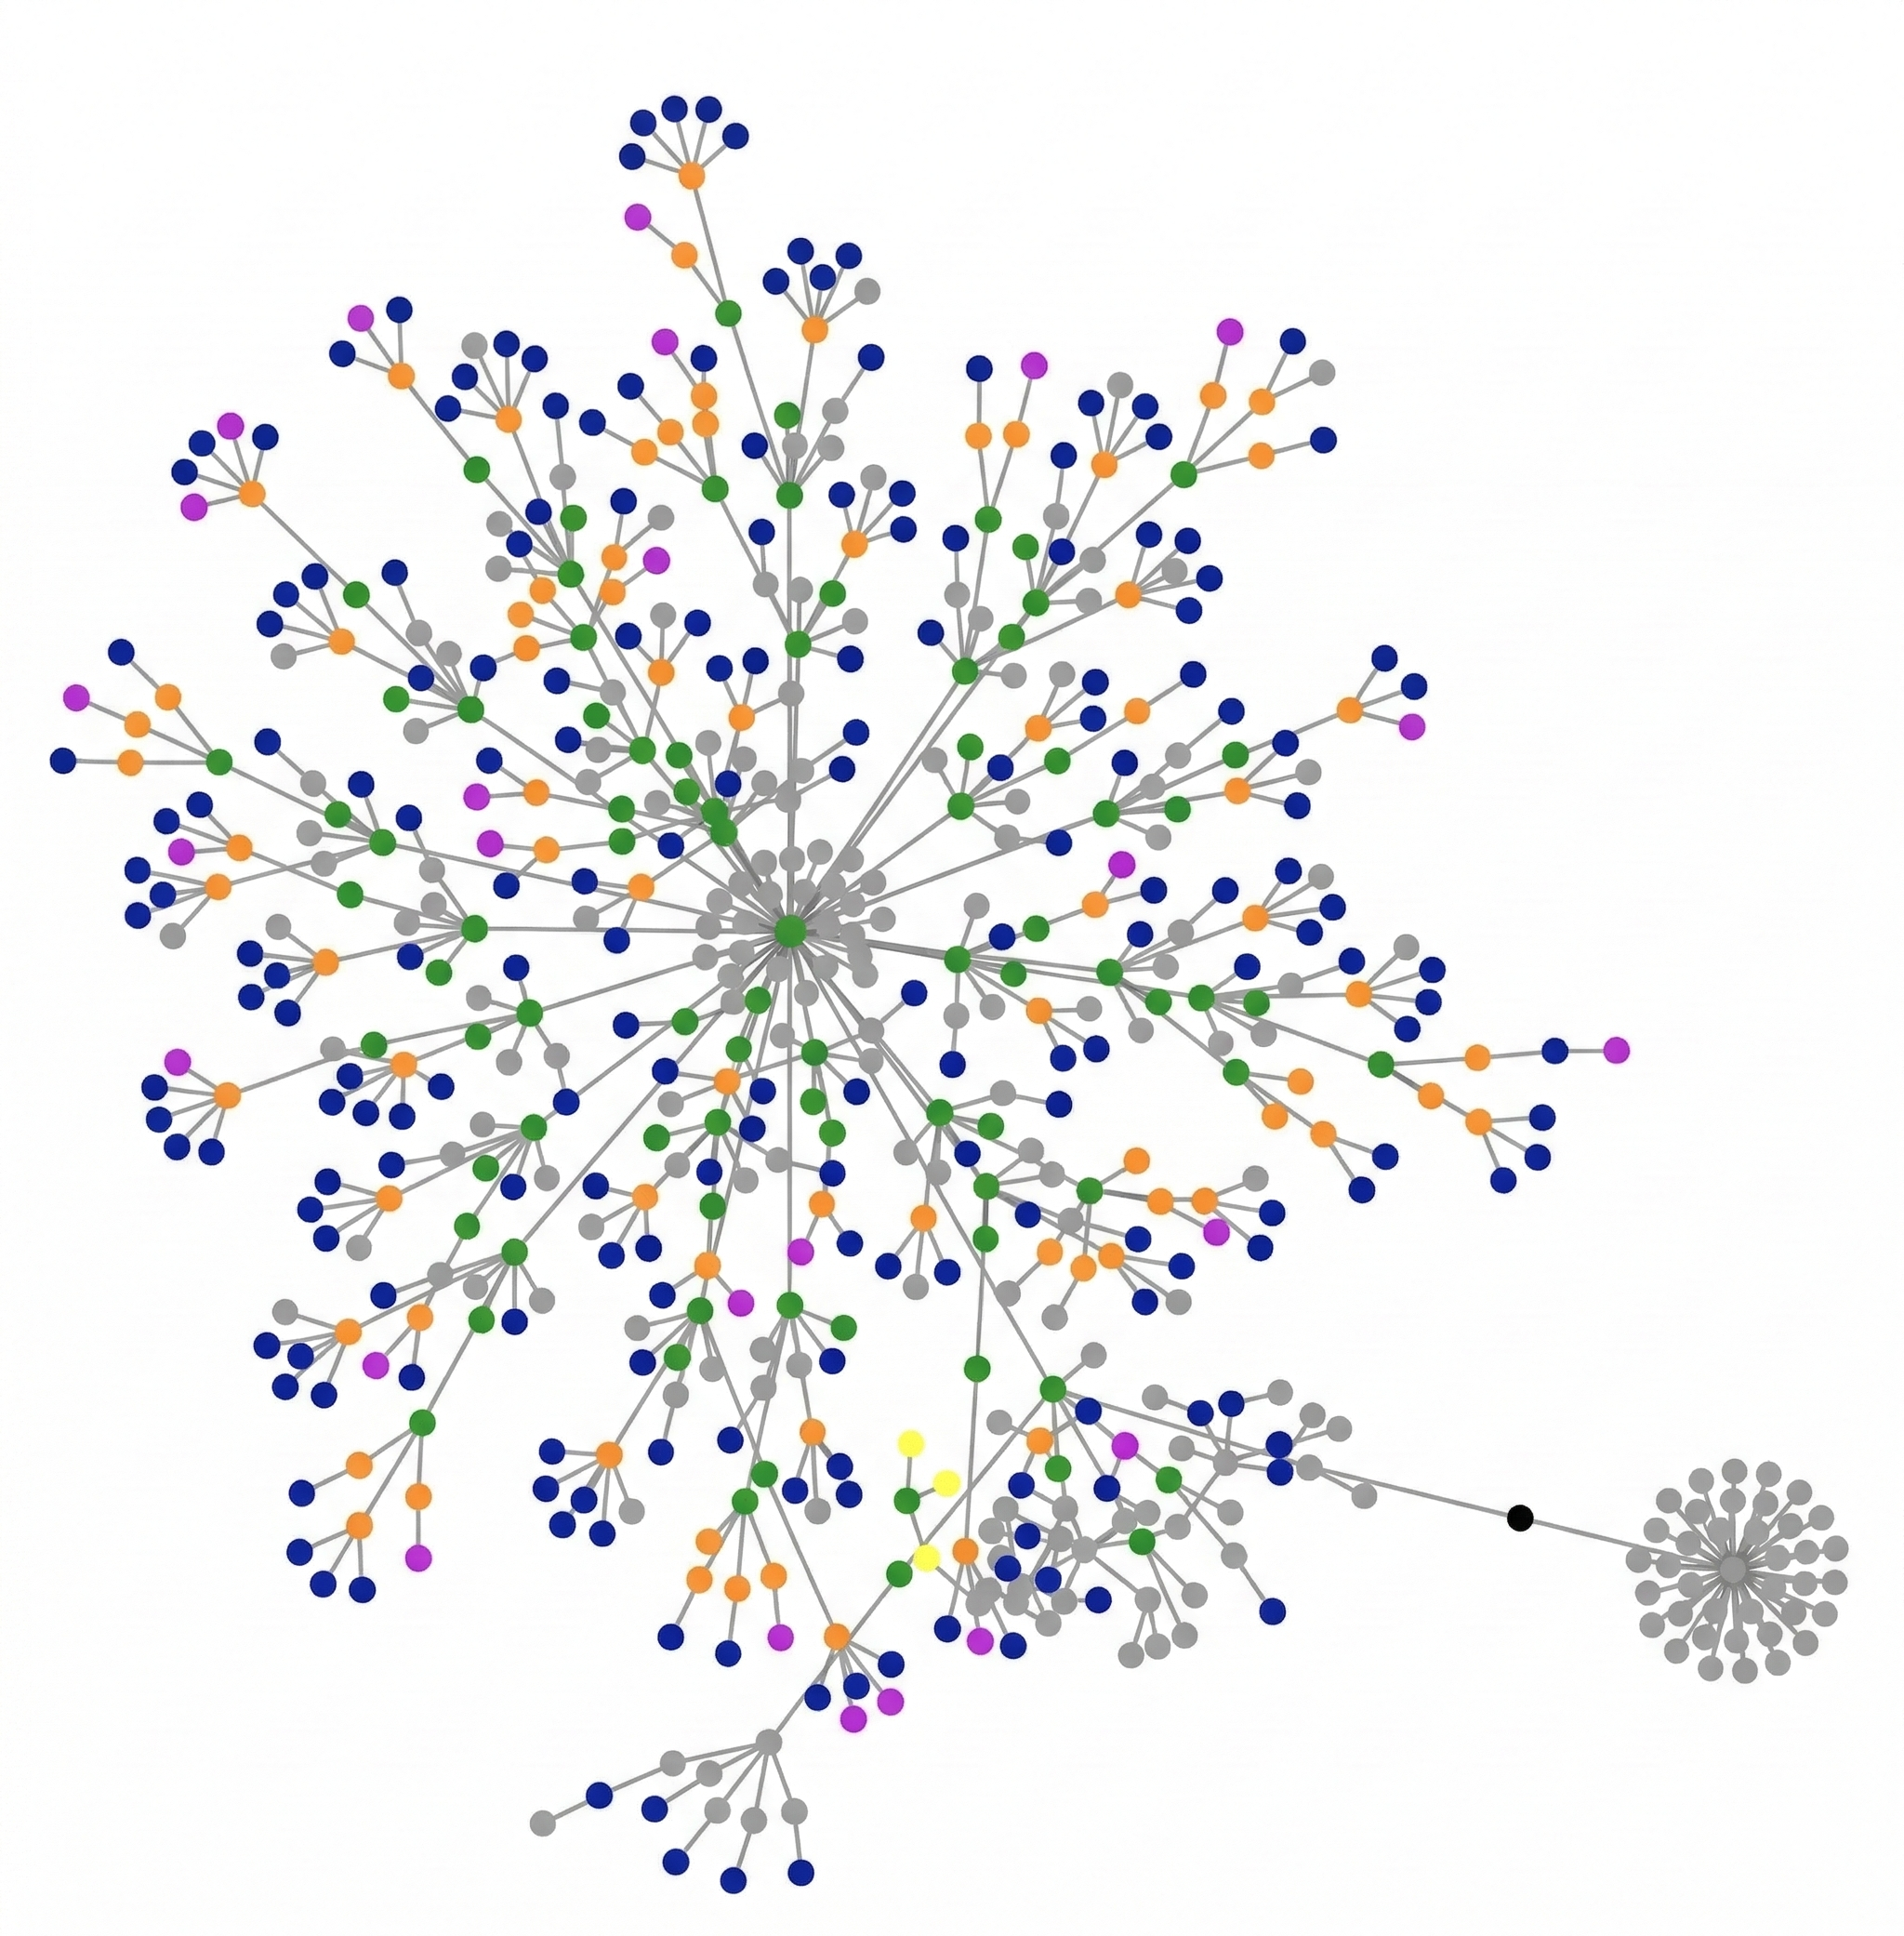
\includegraphics[width=0.9\textwidth]{img/tree_network_example.png}
    \end{minipage}
    \hfill
    \begin{minipage}{0.5\textwidth}
        It is characterized by its branching structure, where each node can have multiple child nodes, but only one parent node. This structure allows for a single path between any two nodes, making it easy to navigate and manage, there  is no redundancy in the connections, which can lead to efficient communication and data transfer. However, it can also lead to bottlenecks if the root node or any intermediate nodes fail, as it can disrupt the entire network.

        \caption{On the left, an example of a tree network, where the central node is the root, and the most external nodes are the leaves. Each node has one parent and can have multiple children, forming a hierarchical structure.}
    \end{minipage}
\end{figure}
With multiple tree networks, it is possible to create a more complex structure, such as a \textbf{forest}, which consists of multiple trees that are not connected to each other. This can provide redundancy and improve the overall resilience of the network.

\begin{example}[Fractals as regular trees.]
    A fractal can be mathematically modeled as a regular tree network. These structures are highly ordered and characterized by specific topological properties: they are self-similar, modular, and deeply hierarchical.

    To understand their spatial properties, we can define two metrics for a tree graph:
    \begin{itemize}
        \item \textbf{Graph Volume ($V$):} The total number of nodes in the network.
        \item \textbf{Graph Surface ($S$):} The number of leaf nodes (nodes with a degree of 1).
    \end{itemize}
    In standard Euclidean geometry (or regular lattices), as an object grows, its surface-to-volume ratio tends to zero ($\lim_{N\to\infty} \frac{S}{V} = 0$). However, fractal networks behave very differently: the number of leaves grows proportionally to the total number of nodes, meaning the surface is directly comparable to the volume ($V \simeq S$). In practical terms, a huge fraction of a fractal tree's nodes are leaves.
\end{example}

\subsection{Directed Acyclic Graph (DAG)}

\begin{minipage}{0.55\textwidth}
    A directed acyclic graph (DAG) is a type of graph that consists of nodes connected by directed edges, where there are no cycles. In a DAG, each edge has a direction, indicating the flow of information or dependencies between nodes. DAGs are commonly used in various applications, such as scheduling tasks, representing dependencies in software development, and modeling hierarchical relationships. It can be used to represent complex systems where there are multiple levels of dependencies, without the risk of creating cycles that can lead to infinite loops or deadlocks.

    With DAGs we can represent more complex relationships than trees, as they allow for multiple paths between nodes, establishing an effective hierarchy. However, they can also be more difficult to manage and navigate, especially as the number of nodes and edges increases. DAGs are often used in scenarios where there are multiple dependencies or relationships between entities, such as in project management, data processing pipelines, and knowledge representation.
\end{minipage}
\hfill
\begin{minipage}{0.4\textwidth}
    \begin{figure}[H]
        \centering
        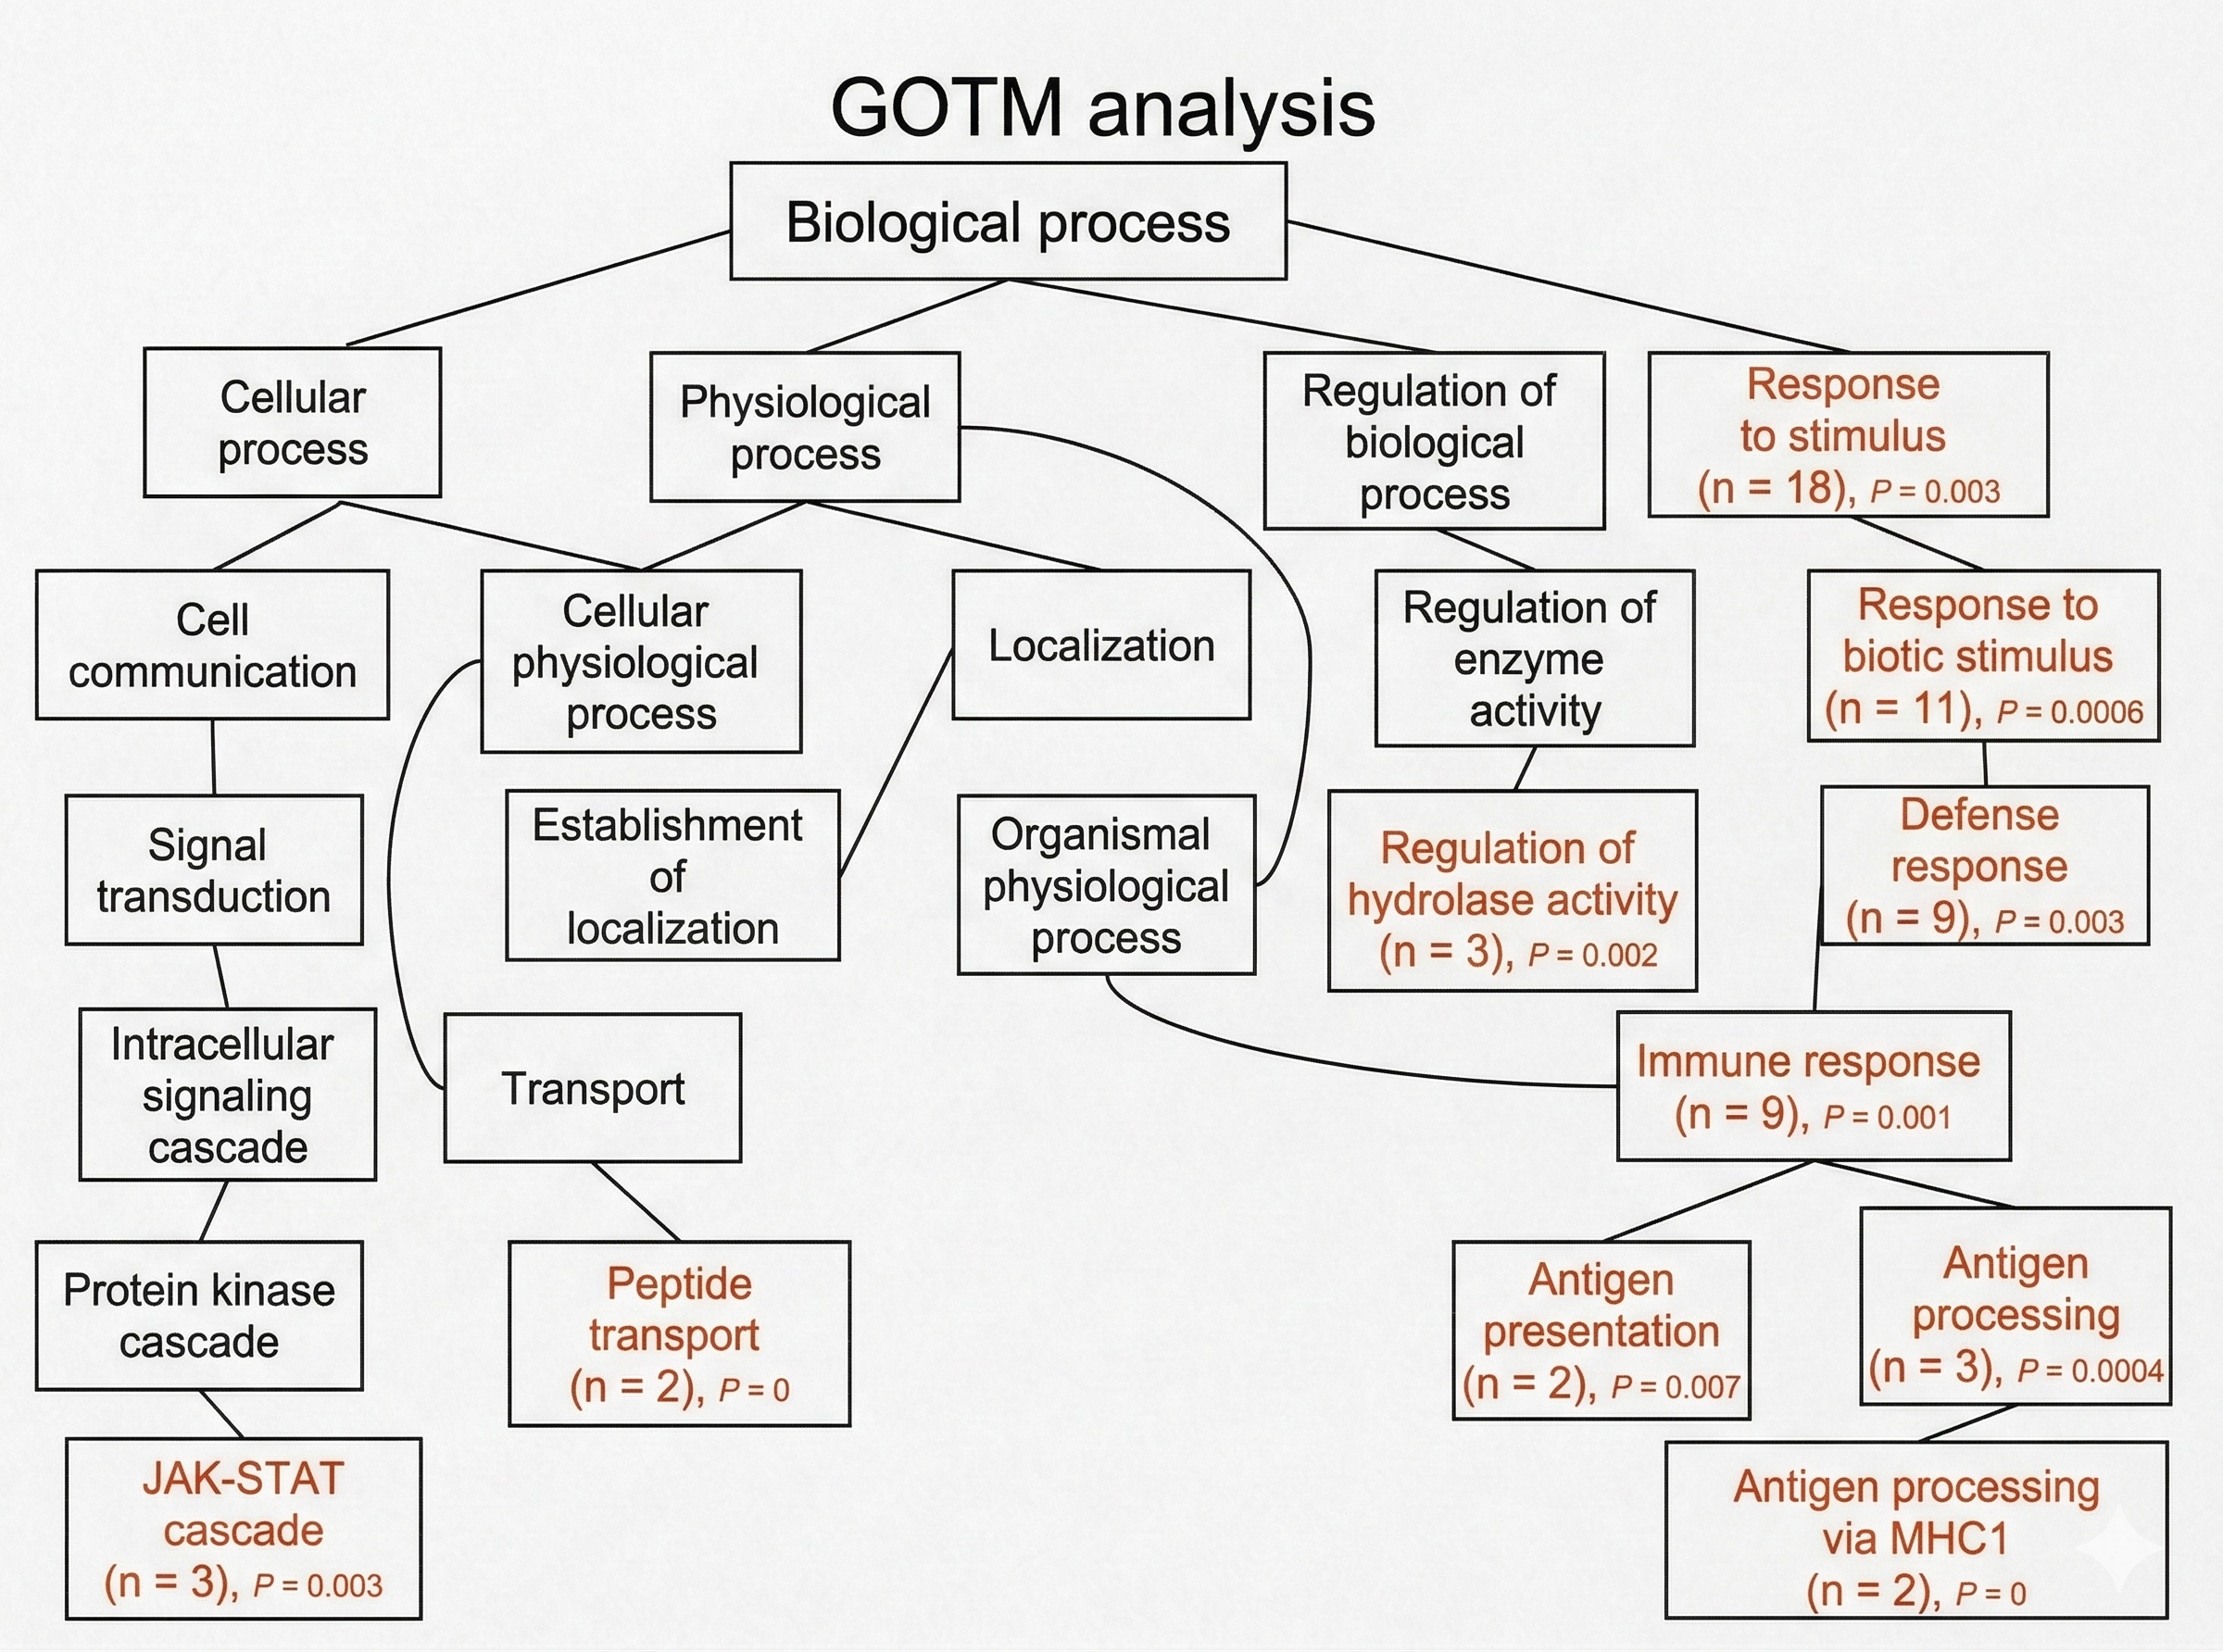
\includegraphics[width=0.9\textwidth]{img/GOTM_analysis_DAG_example.png}
        \caption{An example of a directed acyclic graph (DAG) on the GOTM analysis (which demonstrated that more specific biological processes, such as immune response, regulation of hydrolase activity, peptide transport and JAK-STAT cascade, were significantly modulated by the microbiota; the number of observed genes in a particular biological process is indicated by ``n''). The edges have a direction and there are no cycles. The DAG structure allows for multiple paths between nodes, establishing an effective hierarchy.}
    \end{figure}
\end{minipage}

For networks with these properties, the adjacency matrix is \textbf{upper triangular}, which means that all the entries below the main diagonal are zero. This is because in a DAG, there are no cycles, and therefore, there can be no edges that point back to previous nodes. The upper triangular structure of the adjacency matrix reflects the hierarchical nature of the DAG, where nodes can only have edges pointing to nodes that come after them in the hierarchy. Through this matrix, we can represent the structure of the DAG and analyze its properties as a linear algebra problem, such as finding the longest path or determining the reachability of nodes.